\documentclass{article}
\usepackage{amsmath,  amsthm,  amssymb,  bm,  graphicx, mathrsfs, ctex, caption, subfigure, multicol, multienum, color, float, booktabs}
\usepackage[unicode=true,pdfusetitle,
   bookmarks=true, 
   bookmarksnumbered=false, 
   bookmarksopen=false,
   breaklinks=false, 
   pdfborder={0 0 1}, 
   backref=false, 
   colorlinks=false,
   hidelinks]{hyperref}
\usepackage{anyfontsize}
\usepackage{xeCJK}
\usepackage{geometry}
\usepackage[ruled]{algorithm2e}
\geometry{a4paper, scale=0.8}

\newtheorem*{note}{注}
\newtheorem*{solution}{解}
\newtheorem{theorem}{定理}[section]
\newtheorem{definition}[theorem]{定义}
\newtheorem{lemma}[theorem]{引理}
\newtheorem{corollary}[theorem]{推论}
\newtheorem{example}[theorem]{例} 
\newtheorem{proposition}[theorem]{命题}

\author{杜洪博}
\title{双层优化模型及Benders分解算法讨论分析 \\ {\small 北京邮电大学 优化组}}
\date{\today}


\begin{document}

\maketitle

\section{Benders Decomposition}
\subsection{Unified Primal Subproblems for Benders Decomposition}
\begin{figure}[htbp]
    \centering
    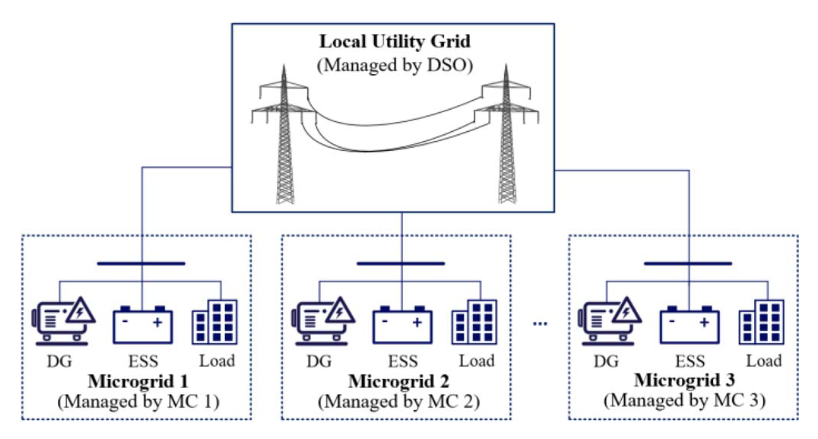
\includegraphics[width=0.8\textwidth]{./pic/NetworkedStructure.png}
    \caption{系统结构示意图}
    \label{fig:structure}
\end{figure}

为了表示方便, 将原始模型以矩阵形式重新表示为如下模型:
\begin{subequations}
    \begin{align}
        \min_{x, y, z}\quad &\mathbf{a}^\mathrm{T}\mathbf{x}+\sum_i\mathbf{b}_i^\mathrm{T}\mathbf{y}_i+\sum_i\mathbf{c}_i^\mathrm{T}\mathbf{z}_i \label{primal_a}\\
        \mathbf{s.t.}\quad & \mathbf{G}(\mathbf{x})\geq\mathbf{d} \label{primal_b} \\
        &\mathbf{B}_{i}\mathbf{x}+\mathbf{C}_{i}\mathbf{y}_{i}+\mathbf{D}_{i}\mathbf{z}_{i}\geq\mathbf{e}_{i}, \forall i \label{primal_c} \\
        &\mathbf{z}_{i}\in\{0, 1\}^{K_{i}}, \forall i \label{primal_d}
    \end{align}
\end{subequations}

根据标准的Benders分解方法, 原问题(\ref{primal_a})-(\ref{primal_d})被划分为一个上层主问题(对应于DSO的决策)和一组下层子问题(对应于个体MCs的决策).主问题表示为:
\begin{subequations}
    \begin{align}
        \min\limits_{\mathbf{x}, \mathbf{\theta}}\quad&\mathbf{a}^\mathrm{T}\mathbf{x}+\sum_i\theta_i \label{master_a}\\
        \mathrm{s.t.}\quad&\mathbf{G}(\mathbf{x})\geq\mathbf{d} \label{master_b}  \\
        &\theta_i\geq0, \forall i \label{master_c}   \\
        &\text{Generated Cutting Planes (if any)} \label{master_d}
    \end{align}
\end{subequations}
其中$\theta_i$为非负连续变量, 用DSO近似表示微电网$i$的运行成本.在每次迭代中, DSO求解主问题, 并将一个试探解$(\hat{\mathbf{x}}, \hat{\theta}_i)$传递给每个MC$(\forall i)$.反过来, 每个MC依次求解两个Benders子问题, 以检验试探解的可行性和最优性, 然后通过Benders割反馈给DSO.可行性子问题为$(\forall i)$:
\begin{subequations}
    \begin{align}
        \min_{y_{i}, z_{i}, s_{i}}\quad& \mathbf{1}^{\mathrm{T}}\mathbf{s}_{i} \label{feasible_a} \\
        \mathbf{s.t.}\quad& \mathbf{C}_i\mathbf{y}_i+\mathbf{D}_i\mathbf{z}_i+\mathbf{s}_i\geq\mathbf{e}_i-\mathbf{B}_i\hat{\mathbf{x}} \label{feasible_b} \\
        &\mathbf{z}_{i}\in\{0, 1\}^{K_{i}}, \mathbf{s}_{i}\geq\mathbf{0} \label{feasible_c}
    \end{align}
\end{subequations}
其中$\mathbf{1}$是一个元素为$1$的向量;$\mathbf{0}$是一个元素为$0$的向量;$s_i$是非负松弛变量的向量.当且仅当(\ref{feasible_a})-(\ref{feasible_c})的最优值为$0$时, 试探解$(\hat{\mathbf{x}}, \hat{\theta_i})$是可行的, 再继续求解最优性子问题(\ref{optimal_a})-(\ref{optimal_c});否则, 将一个可行割返回到主问题, .
\begin{subequations}
    \begin{align}
        \min_{\mathbf{y}_{i}, \mathbf{z}_{i}}\quad& \mathbf{b}_{i}^{\mathrm{T}}\mathbf{y}_{i}+\mathbf{c}_{i}^{\mathrm{T}}\mathbf{z}_{i} \label{optimal_a} \\
        \mathbf{s.t.} \quad&\mathbf{C}_i\mathbf{y}_i+\mathbf{D}_i\mathbf{z}_i\geq\mathbf{e}_i-\mathbf{B}_i\hat{\mathbf{x}} \label{optimal_b} \\
        &\mathbf{z}_{i}\in\{0, 1\}^{K_{i}} \label{optimal_c}
    \end{align}
\end{subequations}

在求解(\ref{optimal_a})-(\ref{optimal_c})后, MC $i$检查得到的解$(\hat{\mathbf{y}}_i, \hat{\mathbf{z}}_i)$, 检查DSO近似的微电网运行成本$\hat{\theta}_i$是否达到$\mathbf{b}_{i}^{\mathrm{T}}\hat{\mathbf{y}}_{i}+\mathbf{c}_{i}^{\mathrm{T}}\hat{\mathbf{z}}_{i}$.如果没有, 则将一个最优割返回到主问题(\ref{master_a})-(\ref{master_d}), 以重新估计微电网运行成本;否则, MC $i$接受试探解$(\hat{\mathbf{x}}, \hat{\theta_i})$, 并且, 如果后续迭代中电力交换计划不变, 则与DSO达成协议.当且仅当所有的MC都与DSO达成协议时, 迭代终止.

可以将两个子问题合并统一表示为如下形式:
\begin{subequations}
    \begin{align}
        \min_{\mathbf{y}_i, \mathbf{z}_i, \mathbf{s}_i}\quad& \mathbf{1}^{\mathrm{T}}\mathbf{s}_{i}+\xi_{i}+\zeta_{i} \label{uni_subproblem_a} \\
        \mathrm{s.t.}\quad&\mathbf{b}_{i}^{\mathrm{T}}\mathbf{y}_{i}+\mathbf{c}_{i}^{\mathrm{T}}\mathbf{z}_{i}+\xi_{i}\geq\hat{\theta}_{i} \label{uni_subproblem_b} \\
        &-\mathbf{b}_i^\mathrm{T}\mathbf{y}_i-\mathbf{c}_i^\mathrm{T}\mathbf{z}_i+\zeta_i\geq-\hat{\theta}_i \label{uni_subproblem_c} \\
        &\mathbf{C}_i\mathbf{y}_i+\mathbf{D}_i\mathbf{z}_i+\mathbf{s}_i\geq\mathbf{e}_i-\mathbf{B}_i\hat{\mathbf{x}} \label{uni_subproblem_d} \\
        &\mathbf{z}_{i}\in\{0, 1\}^{K_{i}}, \mathbf{s}_{i}\geq\mathbf{0}, \xi_{i}, \xi_{i}\geq 0 \label{uni_subproblem_e}
    \end{align}
\end{subequations}
其中, $\xi_i, \zeta_i$为额外的非负松弛变量.当且仅当所有松弛变量$\mathbf{s}_i, \xi_i, \zeta_i$在最优解处都为$0$, MC $i$接受试探解$(\hat{\mathbf{x}}, \hat{\theta_i})$.

主问题(\ref{master_a})-(\ref{master_d})和统一子问题(\ref{uni_subproblem_a})-(\ref{uni_subproblem_e})可以分别表示成如下紧凑的形式:
\begin{subequations}
    \begin{align}
        \min_{\mathbf{x'}}\quad&\mathbf{a'}^{\mathrm{T}}\mathbf{x'} \label{compact_master_a} \\
        \mathrm{s.t.}\quad&\mathbf{H}(\mathbf{x'})\geq\mathbf{d'} \label{compact_master_b} \\
        &\text{Generated Cutting Planes (if any)} \label{compact_master_c}
    \end{align}
\end{subequations}
其中$x'$为$x$中元素与$\theta_i ~ (\forall i)$的聚合, $\mathbf{H}$为定义在$\mathbf{x'}$上的约束.

\begin{subequations}
    \begin{align}
        \min_{\mathbf{y}_{i}, \mathbf{z}_{i}, \mathbf{s}'_{i}}\quad& \mathbf{1}^{\mathrm{T}}\mathbf{s}'_{i} \label{compact_uni_subproblem_a} \\
        \mathbf{s.t.}\quad& \mathbf{C}'{}_i\mathbf{y}_{i}+\mathbf{D}'{}_{i}\mathbf{z}_{i}+\mathbf{s}_{i}'\geq\mathbf{e}'{}_{i}-\mathbf{B}'{}_{i}\mathbf{\hat{x}}' \label{compact_uni_subproblem_b} \\
        &\mathbf{z}_{i}\in\{0, 1\}^{K_{i}}, \mathbf{s}'_i\geq\mathbf{0} \label{compact_uni_subproblem_c}
    \end{align}
\end{subequations}
其中$\mathbf{s}_i'$为$\xi_i,\zeta_i$与$\mathbf{s}_i$中所有元素的聚合.

\subsection{Benders Cuts for Mixed-Integer Linear Subproblems}
通过上述过程可知,统一子问题(\ref{compact_uni_subproblem_a})-(\ref{compact_uni_subproblem_c})是一个混合整数规划问题,常用的基于对偶化的Benders割生成方法无法实现原优化问题(\ref{primal_a})-(\ref{primal_d})可行域的外线性化(outer linearization).

引入辅助01变量向量$\tilde{\mathbf{z}}_i$,限制$\mathbf{z}_i$等于$\tilde{\mathbf{z}}_i$,通过这样的变化,可以将$\mathbf{z}_i$中的所有元素转化为连续变量.即,将(\ref{compact_uni_subproblem_a})-(\ref{compact_uni_subproblem_c})等价转化为如下形式:
\begin{subequations}
    \begin{align}
        \min_{\mathbf{y}_{i},\mathbf{z}_{i},{\tilde{\boldsymbol{z}}}_{i},s'{i}}\quad& \mathbf{1}^{\mathbf{T}}\mathbf{s}'_{i} \label{convert_subproblem_a} \\
        \mathbf{s.t.}\quad & \mathbf{C}_{i}'\mathbf{y}_{i}+\mathbf{D}_{i}'\mathbf{z}_{i}+s_{i}'\geq\mathbf{e}_{i}'-\mathbf{B}'_{i}\hat{\mathbf{x}}'\quad(\bm{\mu}_{i})  \label{convert_subproblem_b} \\
        &\mathbf{z}_{i}=\tilde{\mathbf{z}}_{i}\quad(\bm{\nu}_{i}) \label{convert_subproblem_c} \\
        &\mathbf{s}_{i}'\geq\mathbf{0} \label{convert_subproblem_d} \\
        &\tilde{\mathbf{z}}_{i}\in\{0,1\}^{K_{i}} \label{convert_subproblem_e} 
    \end{align}
\end{subequations}
其中, $\bm{\mu}_i$和$\bm{\nu}_i$分别为(\ref{convert_subproblem_b})和(\ref{convert_subproblem_c})的对偶变量的向量. 然后, 将(\ref{convert_subproblem_a})-(\ref{convert_subproblem_e})重写成以下形式:
\begin{subequations}
    \begin{align}
        \min_{\tilde{\mathbf{z}}_i\in\{0,1\}^{K_i}}\left\{\min_{(y_i,z_i,s'_i)\in P_i}\mathbf{1}^{\text{T}}s'\right\}
        \label{rewrite_convert_subproblem_a}
    \end{align}
其中, $P_i=\{\text{Constraints }(\ref{convert_subproblem_b})-(\ref{convert_subproblem_d})\}$,由于转换掉了$\mathbf{z}_i$的整数约束,所以(\ref{rewrite_convert_subproblem_a})是一个线性规划问题.因此,对内层问题进行对偶化并变换为如下形式:
\begin{align}
    \min_{\tilde{\mathbf{z}}_i\in\{0,1\}^{K_i}}\left\{\max_{(\bm{\mu}_i,\bm{\nu}_i)\in\mathcal{Q}_i}\left\{\left(\mathbf{e}'_i-\mathbf{B}'_i\hat{\mathbf{x}}'\right)^\mathrm{T}\bm{\mu}_i+\tilde{\mathbf{z}}_i^\mathrm{T}\bm{\nu}_i\right\}\right\}
\end{align}
其中, $\mathcal{Q}_i=\{\mathbf{C}_i\bm{\mu}_i=0,\mathbf{D}_i'^{\mathrm{T}}\bm{\mu}_i+\bm{\nu}_i=0,0\leq\bm{\mu}_i\leq 1\}$,根据极小极大不等式,可以得到以下关系:
\begin{align}
    \begin{split}
        \min_{\tilde{\mathbf{z}}_{i}\in\{0,1\}^{K_{i}}} & \left\{\max_{(\bm{\mu}_{i},\bm{\nu}_{i})\in\mathcal{Q}_{i}}\left\{\left(\mathbf{e}'_{i}-\mathbf{B}'_{i}\hat{\mathbf{x}}'\right)^{\mathrm{T}}\bm{\mu}_{i}+\tilde{\mathbf{z}}_{i}^{\mathrm{T}}\bm{\nu}_{i}\right\}\right\}     \\
        & \geq\max_{(\bm{\mu}_{i},\bm{\nu}_{i})\in\mathcal{Q}_{i}}\left\{\min_{\tilde{\mathbf{z}}_{i}\in\{0,1\}^{K_{i}}}\left\{\left(\mathbf{e}_{i}'-\mathbf{B}'_{i}\hat{\mathbf{x}}'\right)^{\mathrm{T}}\bm{\mu}_{i}+\tilde{\mathbf{z}}_{i}^{\mathrm{T}}\bm{\nu}_{i}\right\}\right\}
    \end{split} \label{min_max_inequality}
\end{align}

由于$\tilde{\mathbf{z}}_i$是01变量,所以可以通过枚举$\tilde{\mathbf{z}}_i$的$0$和$1$可能的组合,来确定$\tilde{\mathbf{z}}_{i}^{\mathrm{T}}\bm{\nu}_{i}$的最优值.即:
\begin{align}
    \min_{\tilde{\mathbf{z}}_i\in\{0,1\}^{K_i}}\tilde{\mathbf{z}}_i^\mathrm{T}v_i=\max_{\bm{\omega}_i\in\mathcal{O}_i}\mathbf{1}^\mathrm{T}\bm{\omega}_i
\end{align}
其中, $\mathcal{O}_i=\{\bm{\omega}_i\leq0,\bm{\omega}_i\leq\bm{\nu}_i\}$.于是可以得到(\ref{min_max_inequality})右侧的等价表示:
\begin{align}
    \begin{split}
        \max_{(\bm{\mu}_{i},\bm{\nu}_{i})\in\mathcal{Q}_{i}} & \left\{\left(\mathbf{e}_{i}'-\mathbf{B}'_{i}\hat{\mathbf{x}}'\right)^{\mathrm{T}}\bm{\mu}_{i}+\min_{\tilde{\mathbf{z}}_{i}\in\{0,1\}^{K_{i}}}\tilde{\mathbf{z}}_{i}^{\mathrm{T}}\bm{\nu}_{i}\right\}  \\
        & =\max_{(\bm{\mu}_{i},\bm{\nu}_{i})\in\mathcal{Q}_{i}}\left\{\left(\mathbf{e}_{i}'-\mathbf{B}'_{i}\hat{\mathbf{x}}'\right)^{\mathrm{T}}\bm{\mu}_{i}+\max_{\bm{\omega}_{i}\in\mathcal{O}_{i}}\mathbf{1}^{\mathrm{T}}\bm{\omega}_{i}\right\} 
    \end{split}  \label{max_min_inequality_right}
\end{align}
\end{subequations}
其中, 右侧就变成了一个线性规划问题. 可以该问题将重写为如下形式(记为统一的对偶子问题):
\begin{subequations}
    \begin{align}
        F_{D,i}^*=\max_{(\bm{\mu}_i,\bm{\nu}_i,\bm{\omega}_i)\in\mathcal{Q}_i\cap\mathcal{O}_i}\left\{\left(\mathbf{e}'_i-\mathbf{B}'_i\hat{\mathbf{x}}'\right)^\mathrm{T}\bm{\mu}_i+\mathbf{1}^\mathrm{T}\bm{\omega}_i\right\} \label{rewrite_max_min_inequality_right_a}
    \end{align}
其中, $F_{D,i}^*$为与$\hat{\mathbf{x}}'$有关的最优值, 并且$\bm{\mu}_i$和$\bm{\omega}_i$有最优解$(\hat{\bm{\mu}}_i,\hat{\bm{\omega}}_i)$.

因此, MC $i$ 求解(\ref{rewrite_max_min_inequality_right_a})以检查DSO在每次迭代中传递过来的试探解$\hat{\mathbf{x}}$, 如果$F_{D,i}^*>0$, 则MC $i$ 返回如下的割(记为统一Benders割):
\begin{align}
    \left(\mathbf{e}'_i-\mathbf{B}'_ix'\right)^\mathrm{T}\hat{\bm{\mu}}_i+\mathbf{1}^\mathrm{T}\hat{\bm{\omega}}_i\leq0 \label{uni_benders_cut}
\end{align}
\end{subequations}

\subsection{Feasibility Restoration Cuts for Mitigating Duality Gap}
由于01变量$\tilde{\mathbf{z}}_i$的存在,可能会使得$F_{D,i}^*$与统一原始子问题(\ref{compact_uni_subproblem_a})-(\ref{compact_uni_subproblem_c})之间产生对偶间隙. (\ref{compact_uni_subproblem_a})-(\ref{compact_uni_subproblem_c})的目标函数值为正对应DSO传递的试探解$\hat{\mathbf{x}}'$是不可行的, 这种情况下应当将该试探解割掉. 考虑以下两种情况:
\begin{enumerate}
    \item $F_{D,i}^*$为正, 说明$\hat{\mathbf{x}}'$违反了(\ref{uni_benders_cut}), 当后续迭代(\ref{uni_benders_cut})加入到主问题后, 该试探解将被割掉.
    \item $F_{D,i}^*$非正, 说明$\hat{\mathbf{x}}'$没有违反(\ref{uni_benders_cut}), 此时(\ref{uni_benders_cut})就无法割掉该试探解, 且后续迭代中主问题的最优解就会被卡在$\hat{\mathbf{x}}'$处. 也就是说, 统一Benders割还不够紧.
\end{enumerate}

为了解决第二种情况, 必要时MC $i$ 在求解统一对偶子问题后, 还需要求解如下可行性恢复子问题:
\begin{subequations}
    \begin{align}
        F_{F,i}^{*}=\min_{\mathbf{x',y_{i},z_{i}}} \quad & \Delta_i(\mathbf{x}',\hat{\mathbf{x}}') \label{Feasibility_Restoration_a} \\
        \mathbf{s.t.} \quad& \mathbf{B}_{i}'\mathbf{x}'+\mathbf{C}_{i}\mathbf{y}_i'+\mathbf{D}_{i}'\mathbf{z}_{i}\geq\mathbf{e}_{i}' \label{Feasibility_Restoration_b} \\
        &\mathbf{z}_{i}\in\{0,1\}^{K_{i}}   \label{Feasibility_Restoration_c}
    \end{align}
其中$\Delta_i(\mathbf{x}',\hat{\mathbf{x}}')$表示试探解$\hat{\mathbf{x}}'$与满足(\ref{Feasibility_Restoration_b})-(\ref{Feasibility_Restoration_c})的任意解之间可行性违反程度的度量, 如下所示:
\begin{align}
    \Delta_i(\mathbf{x'},\hat{\mathbf{x}}')=\sum_h\frac{\left|x_h^{\prime}-\hat{x}'_h\right|}{\vartheta_h} \label{Feasibility_Restoration_d}
\end{align}
其中$x_h'$和$\hat{x}_h'$分别为$\mathbf{x}'$和$\hat{\mathbf{x}}'$中的元素, $h$为元素的索引, $\vartheta_h$为与$\hat{x}_h'$相关的归一化因子, 如下所示:
\begin{align}
    \vartheta_h=\begin{cases}|\hat{x}_h^{\prime}|,&if\left|\hat{x}_h^{\prime}\right|>0\\\tau,&if\left|\hat{x}_h^{\prime}\right|=0\end{cases},\forall h \label{Feasibility_Restoration_e}
\end{align}
其中$\tau$是一个足够小的正数. 引入一个辅助连续变量$\sigma_h$来表示$\left|x_h^{\prime}-\hat{x}'_h\right|$, 并将(\ref{Feasibility_Restoration_d})重写为如下形式:
\begin{align}
    \Delta_i(\mathbf{x}',\hat{\mathbf{x}}')=\sum_h\frac{\sigma_h}{\vartheta_h} \label{Feasibility_Restoration_f}
\end{align}
并受到如下约束的限制:
\begin{align}
    \sigma_h&\ge x'_h-\hat{x}'_h,\sigma_h\ge\hat{x}'_h-x'_h,\forall h \label{Feasibility_Restoration_g} \\
    \sigma_h&\le\hat{x}'_h-x'_h+M\delta_h,\sigma_h\le x'_h-\hat{x}'_h+M(1-\delta_h),\forall h   \label{Feasibility_Restoration_h} 
\end{align}
为了使(\ref{Feasibility_Restoration_d})中的绝对值表达式更容易处理, 引入$\delta_h$和$M$, 其中$\delta_h$是辅助01变量, $M$是一个足够大的正数.

在求解可行性恢复子问题(\ref{Feasibility_Restoration_a})-(\ref{Feasibility_Restoration_c})后, 在后续迭代中, 将如下割平面(记为可行性恢复割)和统一Benders割一并加入的主问题中:
\begin{align}
    \Delta_i(\mathbf{x'},\mathbf{\hat{x}'})\geq F_{F,i}^* \label{Feasibility_Restoration_cut}
\end{align}
\end{subequations}

\subsection{Iteration Process}
\begin{figure}[htbp]
    \centering
    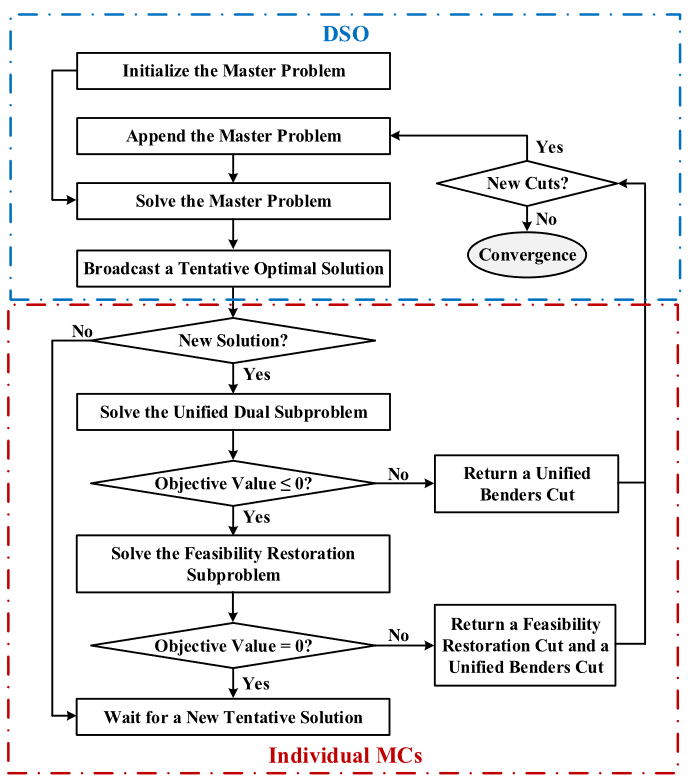
\includegraphics[width=0.8\textwidth]{./pic/IterationProcess.png}
    \caption{迭代过程示意图}
    \label{fig:iteration_process}
\end{figure}


\clearpage
\setcounter{page}{1}
\setcounter{section}{0}

\section{文档所给的双层问题及对部分非线性约束的线性化}
\subsection{上层模型}
\subsubsection{上层目标函数}
以多能互补系统等年值下的系统总投资最小为优化目标:
\setcounter{equation}{0}
\begin{align}
    \min\left(C_{cap}+C_{o\&m}+C_{dep}\right)
\end{align}
式中, $C_{cap}$为系统等年值下的总投资成本, $C_{o\&m}$为系统年运维成本, $C_{dep}$为系统折旧成本.

系统等年值下的总投资成本计算方式如下:
\begin{align}
    C_{cap}=\sum_{k=1}^4C_{cap,k}\cdot\frac{r(1+r)^m}{(1+r)^m-1}
\end{align}
式中, $r$为折现率, $m$为设备的使用年限, $C_{cap,k}$分别为风电、光伏、储能电池逆变器、储能电池装置、光热、储热装置投资成本.
\begin{align}
    \begin{cases}C_{cap,1}=C_W\cdot\lambda_W\\C_{cap,2}=C_V\cdot\lambda_V\\C_{cap,3}=C_B\cdot\lambda_{B_1}+E_B\cdot\lambda_{B_2}\\C_{cap,4}=C_S\cdot\lambda_{S_1}+E_S\cdot\lambda_{S_2}\end{cases}
\end{align}
式中, 所有的$C, E$均为优化变量.

系统运维成本和折旧成本计算方式如下:
\begin{align}
    \begin{cases}C_{o\&m}=C_{cap}\cdot\gamma_o\\C_{dep}=\dfrac{C_{cap}(1-\gamma_r)}m\end{cases}
\end{align}


\subsubsection{上层约束条件}
\begin{enumerate}
    \item 界约束
    \begin{align}
        \begin{cases}0\le C_W\le C_W^{\max}\\0\le C_V\le C_V^{\max}\\0\le C_B\le C_B^{\max}\\0\le E_B\le E_B^{\max}\\0\le C_S\le C_S^{\max}\\0\le E_S\le E_S^{\max}\end{cases}
    \end{align}
    \item {\color{red}储能时长约束}
    \begin{align}
        \begin{cases}E_B=N_B\cdot C_B\\N_B\geq\underline{N}_B\end{cases}
    \end{align}
    式中, $N_B$表示储能电站的储能时长, 为整数优化变量.
\end{enumerate}

\subsection{下层模型}
\subsubsection{下层目标函数}
以等年值下的系统收益最大为优化目标:
\begin{equation}
    \max I
\end{equation}
系统年综合收益为售电收益, 计算方式如下:
\begin{align}
    \begin{cases}
        I=I_E\\
        I_{E}=\lambda_{E}\cdot\sum_{t=1}^{T}p_{L}(t){\cdot}\Delta t
    \end{cases}
\end{align}

\subsubsection{下层约束条件}
下层模型考虑的约束条件包括系统安全性约束和清洁性约束,以及各类装置的运行约束, 现选取部分约束条件进行分析.

\begin{enumerate}
    \item {外送通道容量约束:
        \begin{align}
            p_L(t)&=p_W(t)+p_V(t)+p_B(t)+p_S(t),\forall t\\p_L^{\min}&\le p_L(t)\le p_L^{\max},\forall t
        \end{align}
    }
    \item {风电/光伏运行约束:
        \begin{enumerate}
            \item {发电功率范围约束:
                \begin{align}
                    \begin{cases}0\leq p_W(t)\leq\delta_W(t)\cdot C_W\\0\leq p_V(t)\leq\delta_V(t)\cdot C_V\end{cases},\forall t
                \end{align}
            }
            \item {利用率约束:
                \begin{align}
                    \sum_{t\in\Theta}\left(p_W(t)+p_V(t)\right)\geq(1-\varepsilon)\cdot\sum_{t\in\Theta}\left(\delta_W(t)C_W+\delta_V(t)C_V\right)
                \end{align}
            }
        \end{enumerate}
    }
    \item {储能电站运行约束:
        \begin{enumerate}
            \item {充电功率范围约束({\color{red}可线性化}):
                \begin{align}
                    & p_{B}(t)=p_{B}^{dc}(t)-p_{B}^{ch}(t) \\
                    & \begin{cases}0\leq p_B^{dc}(t)\leq u_B^{dc}(t)\cdot C_B\\0\leq p_B^{ch}(t)\leq u_B^{ch}(t)\cdot C_B\end{cases},\forall t \label{eq:charge_power_range} 
                \end{align}
                式(\ref{eq:charge_power_range})线性化后的约束条件为:
                \begin{align}
                    \begin{cases}
                        0\leq p_B^{dc}(t)\leq u_B^{dc}(t)\cdot C_B^{max}\\
                        0\leq p_B^{ch}(t)\leq u_B^{ch}(t)\cdot C_B^{max}\\
                        0\leq p_B^{dc}(t)\leq C_B\\
                        0\leq p_B^{ch}(t)\leq C_B
                    \end{cases},\forall t
                \end{align}
            }
            \item {充放电状态约束:
                \begin{align}
                    u_B^{dc}(t)+u_B^{ch}(t)\leq1,\forall t
                \end{align}
            }
            \item {荷电状态约束:
                \begin{align}
                    e_B(t+1){=}e_B(t){+}\gamma_B^{ch}p_B^{ch}(t){-}p_B^{dc}(t)/\gamma_B^{dc},\forall t
                \end{align}
            }
            \item {储能容量范围约束:
                \begin{align}
                    0\leq e_B(t)\leq E_B,\forall t
                \end{align}
            }
        \end{enumerate}
    }
    \item {光热电站及储热系统运行约束:
        \begin{enumerate}
            \item {集热器热量平衡约束:
                \begin{align}
                    h_{s}^{in}(t)=h_{s}^{cr}(t)+h_{s}^{ch}(t),\forall t
                \end{align}
            }
            \item {储热/放热功率范围约束:
                \begin{align}
                    \begin{cases}0\le h_S^{ch}(t)\le\bar{h}_S^{ch}\\0\le h_S^{dc}(t)\le\bar{h}_S^{dc}\end{cases},\forall t
                \end{align}
            }
            \item {热-电功率转化约束:
                \begin{align}
                    p_s(t)=\eta_s\cdot h_s(t),\forall t
                \end{align}
            }
            \item {发电功率范围约束({\color{red}可线性化}):
                \begin{align}
                    u_{S}(t)\cdot\delta_{S}^{\min}\cdot C_{S}\leq p_{S}(t)\leq u_{S}(t)\cdot\delta_{S}^{\max}\cdot C_{S},\forall t \label{eq:power_range}
                \end{align}
                式(\ref{eq:power_range})线性化后的约束条件为:
                \begin{align}
                    \begin{cases}
                        u_{S}(t)\cdot\delta_{S}^{\min}\cdot C_{S}^{min}\leq p_{S}(t)\leq u_{S}(t)\cdot\delta_{S}^{\max}\cdot C_{S}^{max}\\
                        \delta_{S}^{\min}\cdot C_{S} - M \cdot (1-u_{S}(t)) \leq p_{S}(t)\leq \delta_{S}^{\max}\cdot C_{S}
                    \end{cases},\forall t
                \end{align}
            }
            \item {发电热量平衡约束:
                \begin{align}
                    h_S^{dc}(t)=h_S(t)+v_S(t)\cdot h_S^g,\forall t
                \end{align}
            }
            \item {运行状态逻辑约束:
                \begin{align}
                    \begin{cases}u_S(t)-u_S(t-1)-\nu_S(t)\leq0\\u_S(t)-\nu_S(t)\geq0\end{cases},\forall t
                \end{align}
            }
            \item {储热装置容量范围约束:
                \begin{align}
                    0\leq e_S(t)\leq E_S,\forall t
                \end{align}
            }
            \item {储热装置热量平衡约束:
                \begin{align}
                    e_S(t+1)=e_S(t)+\gamma_S^{ch}h_S^{ch}(t)-h_S^{dc}(t)/\gamma_S^{dc}-h_S^{l}(t),\forall t
                \end{align}
            }
            \item {储热装置外送能力范围约束:
                \begin{align}
                    0\leq h_S^l(t)\leq\bar{h}_S^l,\forall t
                \end{align}
            }
        \end{enumerate}
    }
    \item {储能装置与风电/光伏弃电状态的耦合运行策略和约束:
        \begin{enumerate}
            \item {风电/光伏弃电状态约束({\color{red}可线性化}):
                \begin{align}
                    \left(1-x(t)\right)\cdot\left(\overline{p}_W(t)+\overline{p}_V(t)\right)\leq p_W(t)+p_V(t)\leq\left(2-x(t)\right)\cdot\left(\overline{p}_W(t)+\overline{p}_V(t)\right)-m,\forall t\in\Theta \label{eq:abandon_power_range}
                \end{align}
                式(\ref{eq:abandon_power_range})线性化后的约束条件为:
                \begin{align}
                    \begin{cases}
                        \left(\overline{p}_W(t)+\overline{p}_V(t)\right)-x(t)\cdot M \leq p_W(t)+p_V(t)\leq 2\cdot\left(\overline{p}_W(t)+\overline{p}_V(t)\right)-m\\
                        0 \leq p_W(t)+p_V(t)\leq\left(\overline{p}_W(t)+\overline{p}_V(t)\right)-m+(1-x(t))\cdot M
                    \end{cases},\forall t\in\Theta
                \end{align}
            }
            \item {储能电站的运行策略约束({\color{red}可线性化}):
                \begin{align}
                    \begin{cases}0\leq p_B^{dc}\left(t\right)\leq\left(1-x(t)\right)\cdot C_B\\0\leq p_B^{ch}\left(t\right)\leq x(t)\cdot C_B&\end{cases},\forall t\in\Theta \label{eq:charge_power_range2_}
                \end{align}
                式(\ref{eq:charge_power_range2_})线性化后的约束条件为:
                \begin{align}
                    \begin{cases}
                        0\leq p_B^{dc}\left(t\right)\leq\left(1-x(t)\right)\cdot C_B^{max}\\
                        0\leq p_B^{ch}\left(t\right)\leq x(t)\cdot C_B^{max}\\
                        0\leq p_B^{dc}\left(t\right)\leq C_B\\
                        0\leq p_B^{ch}\left(t\right)\leq C_B
                    \end{cases},\forall t\in\Theta
                \end{align}
            }
        \end{enumerate}
    }
\end{enumerate}

\section{对所给双层问题的讨论}
\subsection{双层规划的一般形式}
双层规划问题的一般形式如下, 即一个优化问题被另一个优化问题所约束:
\begin{align}
    \min_{x\in X}\quad & f_1(x,y^{*})&  \\
    \mathrm{s.t.}\quad &g_{1}(x,y^{*})\leq0&  \\
    &h_{1}(x,y^{*})=0& \\
    &y^*\in\mathop{\arg\min_{y\in Y}}\{f_2(x,y) \\
    &\qquad~\mathrm{s.t.}~~~~\quad g_{2}(x,y)\leq0\\
    &~~~~~~~~~~~~~~~~~~h_2(x,y)=0\}
\end{align}
% \begin{align}
%     \min_{x\in X,y}\quad&F(x,y)\\
%     \mathrm{s.t.}\quad&G(x,y)\geq0,\\
%     &y\in S(x),
% \end{align}
% 其中, $S(x)$是下面以$x$为参数的优化问题的最优解集。
% \begin{align}
%     \min_{y\in Y}\quad&f(x,y)\\
%     \mathrm{s.t.}\quad&g(x,y)\geq0.
% \end{align}
一般来说下层的决策会影响上层的决策结果。以下为双层规划的一般解法示意图:
\begin{figure}[H]
    \centering
    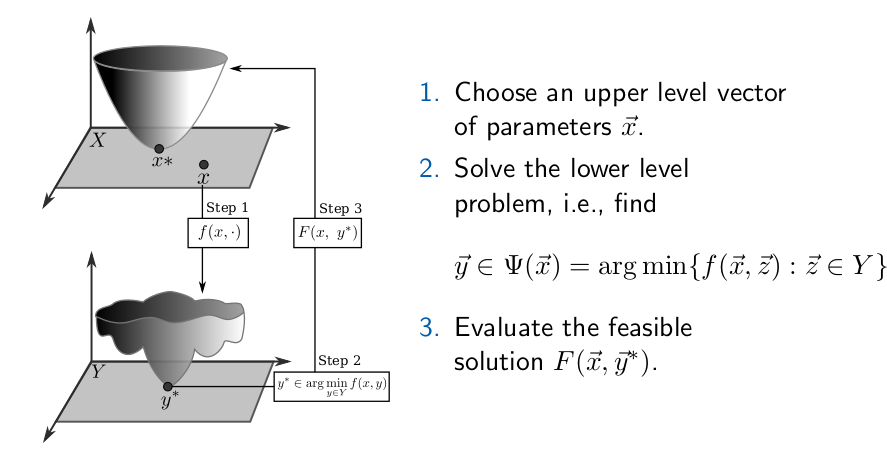
\includegraphics[width=1\textwidth]{./pic/bi-level-scheme.png}
    \caption{双层规划示意图}
    \label{fig:two_level_programming}
\end{figure}
\subsection{文档所给双层问题的矩阵表示}
\begin{enumerate}
    \item {上层问题:
        \begin{align}
            \min\limits_{\boldsymbol{x}\in\boldsymbol{X}}\quad & \boldsymbol{g}^T\boldsymbol{x}  \label{UL_obj} \\
            \mathrm{s.t.}\quad &\boldsymbol{G(x)}\geq \boldsymbol{d}  \label{UL_con1} 
        \end{align}
    }
    \item {下层问题:
        \begin{align}
            \min\limits_{\boldsymbol{y}\in\boldsymbol{F(x)}}\quad & \boldsymbol{h}^T\boldsymbol{y} \\
            \mathrm{s.t.}\quad &\boldsymbol{Bx}+\boldsymbol{Cy}\geq \boldsymbol{e}
        \end{align}
        其中, $\boldsymbol{F(x)}$为下层可行域.
    }
\end{enumerate}

对于这个双层问题, 根据双层规划的一般解法, 可以假设上层问题传入下层问题的$\boldsymbol{x}=\boldsymbol{\hat{x}}$, 不妨设$\boldsymbol{\hat{x}}$传入下层问题后下层问题是可行的。

$\boldsymbol{\hat{x}}$传入下层问题后可得如下形式的下层问题:
\begin{align}
    \min\limits_{\boldsymbol{y}\in\boldsymbol{F(\hat{x})}}\quad & \boldsymbol{h}^T\boldsymbol{y} \\
    \mathrm{s.t.}\quad &\boldsymbol{B\hat{x}}+\boldsymbol{Cy}\geq \boldsymbol{e}
\end{align}
假设此问题的最优解为$\boldsymbol{y^*}$, 将$\boldsymbol{y^*}$传回上层问题, 结合$\boldsymbol{\hat{x}}$, 就获取到了一个上层问题的可行解$(\boldsymbol{\hat{x}},\boldsymbol{y^*})$, 通过这种方式就可以获取到上层问题的所有可行解, 从而可以求解上层问题.

但\eqref{UL_obj}所表示的上层问题的目标函数中并没有$\boldsymbol{y}$, 因此上层问题的最优值与$\boldsymbol{y}$没有关系, 所以这个双层问题可能并不能完成本来的目的。

故而考虑, 将下层问题的目标函数加入到上层问题的目标函数中, 从而得到如下形式新的双层问题:
\begin{enumerate}
    \item {上层问题:
        \begin{align}
            \min\limits_{\boldsymbol{x}\in\boldsymbol{X}}\quad & \boldsymbol{g}^T\boldsymbol{x}+\boldsymbol{h}^T\boldsymbol{y}  \label{UL_obj2} \\
            \mathrm{s.t.}\quad &\boldsymbol{G(x)}\geq \boldsymbol{d}  \label{UL_con12}
        \end{align}
        其中, $\boldsymbol{y}$取值范围为下层问题的最优解集.
    }
    \item {下层问题:
        \begin{align}
            \min\limits_{\boldsymbol{y}\in\boldsymbol{F(x)}}\quad & \boldsymbol{h}^T\boldsymbol{y} \\
            \mathrm{s.t.}\quad &\boldsymbol{Bx}+\boldsymbol{Cy}\geq \boldsymbol{e}
        \end{align}
        其中, $\boldsymbol{F(x)}$为下层可行域.
    }
\end{enumerate}

\subsection{单层问题}
以下为所给文档中给出的单层问题:
\begin{figure}[H]
    \centering
    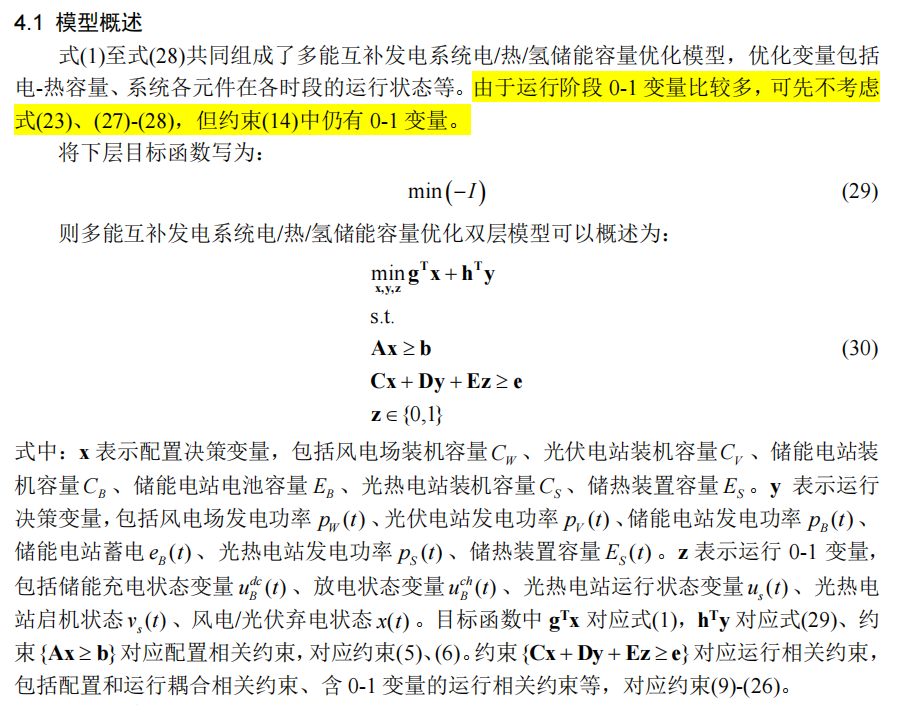
\includegraphics[width=0.8\textwidth]{./pic/单层问题.png}
    \caption{单层问题}
    \label{fig:single_level_programming}
\end{figure}
为了表述简洁这里将下层问题中的变量统一使用$\boldsymbol{y}$表示, 不特意区分01变量和连续变量.
\begin{align}
    \min\limits_{\boldsymbol{x,y}\in\boldsymbol{F(x,y)}}\quad & \boldsymbol{g}^T\boldsymbol{x}+\boldsymbol{h}^T\boldsymbol{y}\\
    \mathrm{s.t.}\quad &\boldsymbol{G(x)}\geq \boldsymbol{d} \\
    &\boldsymbol{Bx}+\boldsymbol{Cy}\geq \boldsymbol{e}
\end{align}
其中, $\boldsymbol{F(x,y)}=\{(\boldsymbol{x,y})|\boldsymbol{x}\in\boldsymbol{X},\boldsymbol{y}\in\boldsymbol{F(x)}\}$.

\subsection{证明新的双层问题与单层问题的最优值相同}
要证:
\begin{align}
    \min\limits_{\boldsymbol{x}\in\boldsymbol{X}}\min\limits_{\boldsymbol{y}\in\boldsymbol{F(x)}} (\boldsymbol{g}^T\boldsymbol{x}+ \boldsymbol{h}^T\boldsymbol{y})=\min\limits_{\boldsymbol{x,y}\in\boldsymbol{F(x,y)}}(\boldsymbol{g}^T\boldsymbol{x}+\boldsymbol{h}^T\boldsymbol{y}) \label{eq:proof}
\end{align}
\eqref{eq:proof}可以表示为:
\begin{align}
    \min\limits_{\boldsymbol{x}\in\boldsymbol{X}}\min\limits_{\boldsymbol{y}\in\boldsymbol{F(x)}} f(\boldsymbol{x,y})=\min\limits_{\boldsymbol{x,y}\in\boldsymbol{F(x,y)}} f(\boldsymbol{x,y}), \quad \boldsymbol{F(x,y)}=\{(\boldsymbol{x,y})|\boldsymbol{x}\in\boldsymbol{X},\boldsymbol{y}\in\boldsymbol{F(x)}\}
\end{align}
\begin{enumerate}
    \item 假设$(\boldsymbol{x^*,y^*})$为$LHS$的最优解, 同时$(\boldsymbol{x^*,y^*})$也是$RHS$的可行解, 则有:
    \begin{align}
        LHS\leq RHS \label{eq:proof1}
    \end{align}
    \item 假设$(\boldsymbol{x^*,y^*})$为$RHS$的最优解, 那么$\min\limits_{\boldsymbol{y}\in F(\boldsymbol{x^*})}f(\boldsymbol{x^*,y})$有最优解$(\boldsymbol{x^*,\widetilde{y}})$, 且有:
    \begin{align}
        f(\boldsymbol{x^*,\widetilde{y}})\geq f(\boldsymbol{x^*,y^*})
    \end{align}
    所以:
    \begin{align}
        LHS\geq RHS \label{eq:proof2}
    \end{align}
\end{enumerate}
综上, 由\eqref{eq:proof1}和\eqref{eq:proof2}可得:
\begin{align}
    LHS=RHS
\end{align}

\section{文章中的Benders分解存在的问题}
文章中只有可行性恢复子问题, 保证了可行性, 但没有保证最优性。

\section{对模型中\texorpdfstring{$E_B=N_B\cdot C_B$}.约束的处理}
初步可以使用枚举的方法进行测试, 通过求解多个MILP问题实现, 即分别令$N_B=\underline{N}_B,\underline{N}_B+1,\cdots$, 求解对应的MILP问题, 并统计各个问题的目标函数值, 选取最优的目标函数值对应的$N_B$值作为最终的$N_B$值.

\section{结论}
\begin{enumerate}
    \item {目前双层模型的本质是单层模型, 单层模型的最优解即为双层模型的最优解。}
    \item {Benders分解适用于单层模型的问题, 且模型分解后的子问题中不应含有整数变量。}
\end{enumerate}

\clearpage

\begin{enumerate}
    \item 第一种形式:
    \begin{align}
        \min_{x\in X}\quad & f(x)+g(y)  \\
        \mathrm{s.t.}\quad &h(x)\leq0  \\
        &y\in\mathop{\arg\max_{y\in Y}}\{u(x,y) \\
        &\qquad~\mathrm{s.t.}~~~\quad k(x,y)\leq0\\
        &~~~~~~~~~~~~~~~~~e(y)+c(x)\leq0\}
    \end{align}

    \item 第二种形式:
    
    上层问题:
    \begin{align}
        \min_{x\in X}\quad & f(x)+g(y)  \\
        \mathrm{s.t.}\quad &h(x)\leq0  \\
        &y\in S(x) 
    \end{align}
    其中, $S(x)$是下面以$x$为参数的下层优化问题的最优解集。
    \begin{align}
        \max_{y\in Y}\quad&u(x,y)\\
        \mathrm{s.t.}\quad&k(x,y)\leq0\\
        &e(y)+c(x)\leq0.
    \end{align}
\end{enumerate}

\clearpage
\setcounter{section}{0}
\section{新双层模型}
\subsection{上层模型}
\subsubsection{上层目标函数}
以多能互补系统等年值下的系统总投资最小为优化目标:
\setcounter{equation}{0}
\begin{align}
    \min~ R=I-\left(C_{cap}+C_{o\&m}+C_{dep}\right)
\end{align}
式中, $R$表示多能互补发电系统的年净收益, $I$表示系统的年综合收益,$C_{cap}$为系统等年值下的总投资成本, $C_{o\&m}$为系统年运维成本, $C_{dep}$为系统折旧成本.

{\color{red}由于全年 8760h 时段数量太多,可以只考虑每个月 1 个典型日场景,全年收益是每个月的天数乘以给定的典型日场景的收益.}

系统年综合收益为售电收益, 计算方式如下:
\begin{align}
    \begin{cases}
        I=I_E\\
        I_{E}=\lambda_{E}\cdot\sum\limits_{t=1}^{T}p_{L}(t){\cdot}\Delta t
    \end{cases}
\end{align}

系统等年值下的总投资成本计算方式如下:
\begin{align}
    C_{cap}=\sum_{k=1}^4C_{cap,k}\cdot\frac{r(1+r)^m}{(1+r)^m-1}
\end{align}
式中, $r$为折现率, $m$为设备的使用年限, $C_{cap,k}$分别为风电、光伏、储能电池逆变器、储能电池装置、光热、储热装置投资成本.
\begin{align}
    \begin{cases}C_{cap,1}=C_W\cdot\lambda_W\\C_{cap,2}=C_V\cdot\lambda_V\\C_{cap,3}=C_B\cdot\lambda_{B_1}+E_B\cdot\lambda_{B_2}\\C_{cap,4}=C_S\cdot\lambda_{S_1}+E_S\cdot\lambda_{S_2}\end{cases}
\end{align}
式中, 所有的$C, E$均为优化变量.

系统运维成本和折旧成本计算方式如下:
\begin{align}
    \begin{cases}C_{o\&m}=C_{cap}\cdot\gamma_o\\C_{dep}=\dfrac{C_{cap}(1-\gamma_r)}m\end{cases}
\end{align}


\subsubsection{上层约束条件}
\begin{enumerate}
    \item 界约束
    \begin{align}
        \begin{cases}0\le C_W\le C_W^{\max}\\0\le C_V\le C_V^{\max}\\0\le C_B\le C_B^{\max}\\0\le E_B\le E_B^{\max}\\0\le C_S\le C_S^{\max}\\0\le E_S\le E_S^{\max}\end{cases}
    \end{align}
    \item {\color{red}储能时长约束}
    \begin{align}
        \begin{cases}E_B=N_B\cdot C_B\\N_B\geq\underline{N}_B\end{cases}
    \end{align}
    式中, $N_B$表示储能电站的储能时长, 为整数优化变量.
\end{enumerate}

\subsection{下层模型}
\subsubsection{下层目标函数}
以系统供电缺额最小为优化目标:
\begin{equation}
    \min\sum_tp_D(t)
\end{equation}
式中, $p_D(t)$表示时刻$t$的系统供电缺额.

\subsubsection{下层约束条件}
下层模型考虑的约束条件包括系统安全性约束和清洁性约束,以及各类装置的运行约束, 现选取部分约束条件进行分析.

\begin{enumerate}
    \item {无故障时外送通道容量约束:
        \begin{gather}
            p_L(t)=p_W(t)+p_V(t)+p_B(t)+p_S(t),\forall t\in\Theta\\
            p_L(t)+p_D(t)\geq p_{LM}(t),\forall t\in\Theta\\
            p_D(t)\geq0,\forall t\in\Theta
        \end{gather}
        式中, $\Theta$表示所有时段集合, $p_{LM}(t)$表示送出功率下限,为给定曲线.
    }
    \item {风电/光伏运行约束:
        \begin{enumerate}
            \item {发电功率范围约束:
                \begin{align}
                    \begin{cases}0\leq p_W(t)\leq\delta_W(t)\cdot C_W\\0\leq p_V(t)\leq\delta_V(t)\cdot C_V\end{cases},\forall t
                \end{align}
            }
            \item {利用率约束:
                \begin{align}
                    \sum_{t\in\Theta}\left(p_W(t)+p_V(t)\right)\geq(1-\varepsilon)\cdot\sum_{t\in\Theta}\left(\delta_W(t)C_W+\delta_V(t)C_V\right)
                \end{align}
            }
        \end{enumerate}
    }
    \item {储能电站运行约束:
        \begin{enumerate}
            \item {充电功率范围约束({\color{red}可线性化}):
                \begin{align}
                    & p_{B}(t)=p_{B}^{dc}(t)-p_{B}^{ch}(t) \\
                    & \begin{cases}0\leq p_B^{dc}(t)\leq u_B^{dc}(t)\cdot C_B\\0\leq p_B^{ch}(t)\leq u_B^{ch}(t)\cdot C_B\end{cases},\forall t \label{eq:charge_power_range2} 
                \end{align}
                式(\ref{eq:charge_power_range2})线性化后的约束条件为:
                \begin{align}
                    \begin{cases}
                        0\leq p_B^{dc}(t)\leq u_B^{dc}(t)\cdot C_B^{max}\\
                        0\leq p_B^{ch}(t)\leq u_B^{ch}(t)\cdot C_B^{max}\\
                        0\leq p_B^{dc}(t)\leq C_B\\
                        0\leq p_B^{ch}(t)\leq C_B
                    \end{cases},\forall t
                \end{align}
            }
            \item {充放电状态约束:
                \begin{align}
                    u_B^{dc}(t)+u_B^{ch}(t)\leq1,\forall t
                \end{align}
            }
            \item {荷电状态约束:
                \begin{align}
                    e_B(t+1){=}e_B(t){+}\gamma_B^{ch}p_B^{ch}(t){-}p_B^{dc}(t)/\gamma_B^{dc},\forall t
                \end{align}
            }
            \item {储能容量范围约束:
                \begin{align}
                    0\leq e_B(t)\leq E_B,\forall t
                \end{align}
            }
        \end{enumerate}
    }
    \item {光热电站及储热系统运行约束:
        \begin{enumerate}
            \item {集热器热量平衡约束:
                \begin{align}
                    h_{s}^{in}(t)=h_{s}^{cr}(t)+h_{s}^{ch}(t),\forall t
                \end{align}
            }
            \item {储热/放热功率范围约束:
                \begin{align}
                    \begin{cases}0\le h_S^{ch}(t)\le\bar{h}_S^{ch}\\0\le h_S^{dc}(t)\le\bar{h}_S^{dc}\end{cases},\forall t
                \end{align}
            }
            \item {热-电功率转化约束:
                \begin{align}
                    p_s(t)=\eta_s\cdot h_s(t),\forall t
                \end{align}
            }
            \item {发电功率范围约束({\color{red}可线性化}):
                \begin{align}
                    u_{S}(t)\cdot\delta_{S}^{\min}\cdot C_{S}\leq p_{S}(t)\leq u_{S}(t)\cdot\delta_{S}^{\max}\cdot C_{S},\forall t \label{eq:power_range2}
                \end{align}
                式(\ref{eq:power_range2})线性化后的约束条件为:
                \begin{align}
                    \begin{cases}
                        u_{S}(t)\cdot\delta_{S}^{\min}\cdot C_{S}^{min}\leq p_{S}(t)\leq u_{S}(t)\cdot\delta_{S}^{\max}\cdot C_{S}^{max}\\
                        \delta_{S}^{\min}\cdot C_{S} - M \cdot (1-u_{S}(t)) \leq p_{S}(t)\leq \delta_{S}^{\max}\cdot C_{S}
                    \end{cases},\forall t
                \end{align}
            }
            \item {发电热量平衡约束:
                \begin{align}
                    h_S^{dc}(t)=h_S(t)+v_S(t)\cdot h_S^g,\forall t
                \end{align}
            }
            \item {运行状态逻辑约束:
                \begin{align}
                    \begin{cases}u_S(t)-u_S(t-1)-\nu_S(t)\leq0\\u_S(t)-\nu_S(t)\geq0\end{cases},\forall t
                \end{align}
            }
            \item {储热装置容量范围约束:
                \begin{align}
                    0\leq e_S(t)\leq E_S,\forall t
                \end{align}
            }
            \item {储热装置热量平衡约束:
                \begin{align}
                    e_S(t+1)=e_S(t)+\gamma_S^{ch}h_S^{ch}(t)-h_S^{dc}(t)/\gamma_S^{dc}-h_S^{l}(t),\forall t
                \end{align}
            }
            \item {储热装置外送能力范围约束:
                \begin{align}
                    0\leq h_S^l(t)\leq\bar{h}_S^l,\forall t
                \end{align}
            }
        \end{enumerate}
    }
    \item {储能装置与风电/光伏弃电状态的耦合运行策略和约束:
        \begin{enumerate}
            \item {风电/光伏弃电状态约束({\color{red}可线性化}):
                \begin{align}
                    \left(1-x(t)\right)\cdot\left(\overline{p}_W(t)+\overline{p}_V(t)\right)\leq p_W(t)+p_V(t)\leq\left(2-x(t)\right)\cdot\left(\overline{p}_W(t)+\overline{p}_V(t)\right)-m,\forall t\in\Theta \label{eq:abandon_power_range_2}
                \end{align}
                式(\ref{eq:abandon_power_range_2})线性化后的约束条件为:
                \begin{align}
                    \begin{cases}
                        \left(\overline{p}_W(t)+\overline{p}_V(t)\right)-x(t)\cdot M \leq p_W(t)+p_V(t)\leq 2\cdot\left(\overline{p}_W(t)+\overline{p}_V(t)\right)-m\\
                        0 \leq p_W(t)+p_V(t)\leq\left(\overline{p}_W(t)+\overline{p}_V(t)\right)-m+(1-x(t))\cdot M
                    \end{cases},\forall t\in\Theta
                \end{align}
            }
            \item {储能电站的运行策略约束({\color{red}可线性化}):
                \begin{align}
                    \begin{cases}0\leq p_B^{dc}\left(t\right)\leq\left(1-x(t)\right)\cdot C_B\\0\leq p_B^{ch}\left(t\right)\leq x(t)\cdot C_B&\end{cases},\forall t\in\Theta \label{eq:charge_power_range2_2}
                \end{align}
                式(\ref{eq:charge_power_range2_2})线性化后的约束条件为:
                \begin{align}
                    \begin{cases}
                        0\leq p_B^{dc}\left(t\right)\leq\left(1-x(t)\right)\cdot C_B^{max}\\
                        0\leq p_B^{ch}\left(t\right)\leq x(t)\cdot C_B^{max}\\
                        0\leq p_B^{dc}\left(t\right)\leq C_B\\
                        0\leq p_B^{ch}\left(t\right)\leq C_B
                    \end{cases},\forall t\in\Theta
                \end{align}
            }
        \end{enumerate}
    }
\end{enumerate}

\section{对所给双层问题的讨论}
\subsection{一般形式}
\begin{align}
    \min_{x\in X}\quad & f_1(x,y)  \\
    \mathrm{s.t.}\quad &g_1(x)\leq0  \\
    &h_1(x)=0\\
    &y\in\mathop{\arg\max_{y\in Y}}\{f_2(y) \\
    &\qquad~\mathrm{s.t.}~~~\quad g_2(x,y)\leq0\\
    &~~~~~~~~~~~~~~~~~h_2(x,y)=0\}
\end{align}
其中, $x$为上层决策变量, 含有整数变量; $y$为下层决策变量, 含有0-1变量; $f_1(x,y)$为上层目标函数, $f_2(y)$为下层目标函数, $g_1(x),h_1(x)$为上层约束条件, 含有非线性项如下所示; $g_2(x,y),h_2(x,y)$为下层约束条件, 都为线性约束.

储能时长约束
\begin{align*}
    \begin{cases}E_B=N_B\cdot C_B\\N_B\geq\underline{N}_B\end{cases}
\end{align*}
式中, $N_B$表示储能电站的储能时长, 为整数优化变量.

\subsection{非线性项处理}
对于上层问题中的非线性项可以采用枚举的方法, 通过求解多个MILP问题实现, 即分别令$N_B=\underline{N}_B,\underline{N}_B+1,\cdots$, 求解对应的MILP问题, 并统计各个问题的目标函数值, 选取最优的目标函数值对应的$N_B$值作为最终的$N_B$值.

枚举后的上层约束条件也都为线性约束, 所得到的新的双层问题就是一个混合整数线性的双层规划问题, 上层问题不含整数变量, 下层问题含有0-1变量.

\subsection{调研结果}
目前求解器可以求解的问题类型有:
\begin{enumerate}
    \item {上下层都为凸(LP-LP、LP-QP、LP-SOCP...)}
    \item {上下层都为整数线性规划(ILP-ILP)}
\end{enumerate}

一种针对MIBLP问题的求解方法, 先将问题转化为如下形式:
\begin{align*}
    \operatorname*{min}_{x,y}c_{x}^{T}x+c_{y}^{T}y \\
    G_{x}x+G_{y}y& \leq q  \\
    Ax+By&\leq b \\
    l\leq y& \leq u  \\
    x_j\text{ integer},&\forall j\in J_x\\
    y_{j}\text{ integer},&\forall j\in J_{y} \\
    d^{T}y&\leq\Phi(x)
\end{align*}
其中$\Phi(x)$为以下值函数:
$$
\Phi(x^*):=\min_{y\in\mathbb{R}^n2}\{d^Ty~:~By\leq b-Ax^*,\quad l\leq y\leq u,\quad y_j\mathrm{~integer~}\forall j\in J_y\}.
$$
去掉约束$d^Ty\leq\Phi(x)$得到High Point Relaxation(HPR).

求解算法如下:
\begin{figure}[H]
    \centering
    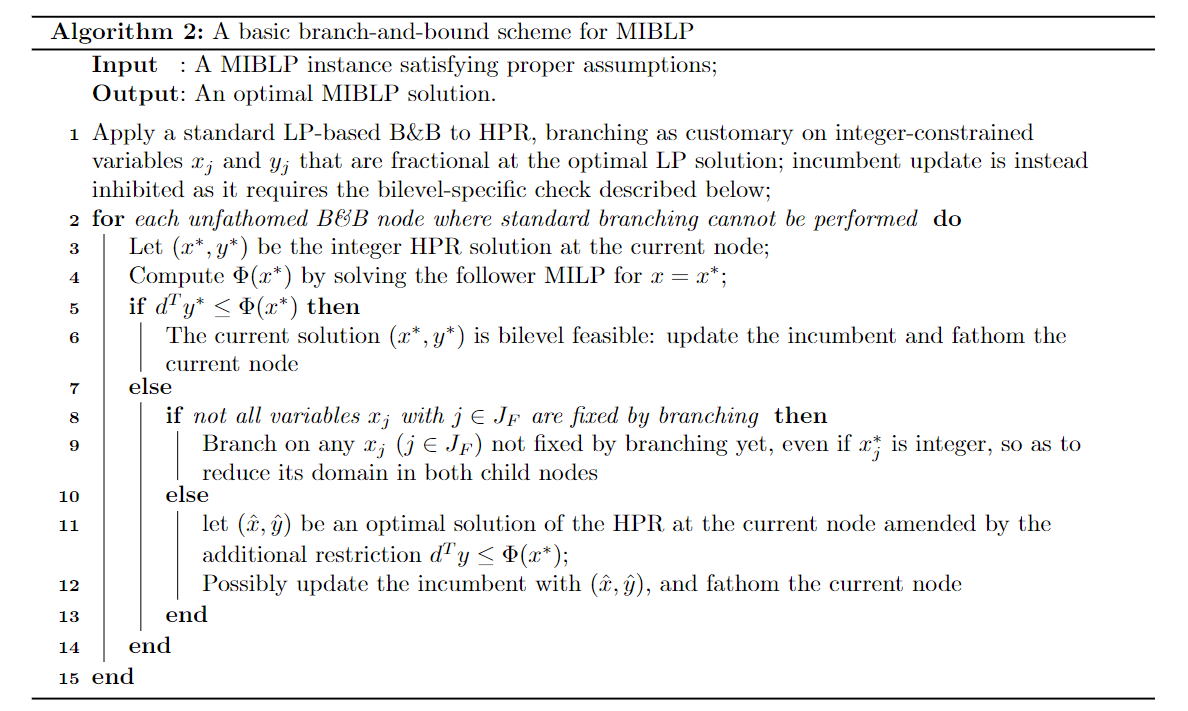
\includegraphics[width=0.9\textwidth]{./pic/MIBLP_algo.png}
    \label{fig:MIBLP}
\end{figure}
Here $J_F$ is the set of the leader x-variables appearing in the follower problem, all of 
which are assumed to be integer constrained (we also exclude HPR unboundedness)

\clearpage

\section{双层模型求解}
\subsection{值函数单层化模型}
\begin{align*}
    \operatorname*{min}_{x,y}c_{x}^{T}x+c_{y}^{T}y \\
    G_{x}x+G_{y}y& \leq q  \\
    Ax+By&\leq b \\
    l\leq y& \leq u  \\
    x_j\text{ integer},&\forall j\in J_x\\
    y_{j}\text{ integer},&\forall j\in J_{y} \\
    d^{T}y&\leq\Phi(x)
\end{align*}
其中$\Phi(x)$为值函数, 表示对于$x$的下层问题的最优值.:
$$
\Phi(x^*):=\min_{y\in\mathbb{R}^n2}\{d^Ty~:~By\leq b-Ax^*,\quad l\leq y\leq u,\quad y_j\mathrm{~integer~},\forall j\in J_y\}.
$$
去掉约束$d^Ty\leq\Phi(x)$得到High Point Relaxation(HPR).

本模型中,值函数为给定$x$的下层问题的最优值$\sum\limits_{t} p_D$。

\subsection{启发式求解算法}

\begin{algorithm}[H]
    \caption{基于分支定界框架的启发式算法}%算法名字
    \LinesNumbered %要求显示行号
    % \KwIn{input parameters A, B, C}%输入参数
    % \KwOut{output result}%输出
    % Apply a standard LP$-$based B$ \& $B to HPR, branching as customary on integer$-$constrained
    % variables $x_j$ and $y_j$ that are fractional at the optimal LP solution\; %\;用于换行
    \While{分支定界Gap未缩减到0}{
        \If{当前节点的解整数可行}{
            令$(x^*,y^*)$为HPR当前节点的整数可行解, 计算代表下层问题的值函数$\Phi(x^*)$\;
            \If{$d^Ty^*\leq \Phi(x^*)$}{
                向原模型中添加Lazy Constraint: $d^Ty\leq \Phi(x^*)$\;
            }
        }
    }
\end{algorithm}

\clearpage
\subsection{数值实验}
计算环境: Intel(R) Core(TM) i5-8300H CPU @ 2.30GHz, 16GB内存, Windows 10操作系统, Julia v1.8, Gurobi v11.0.0rc2.

 1. HPR求解结果:
\begin{table}[H]
    \centering
    \caption{HPR求解结果}
    \label{tab:energy_system_data}
    \begin{tabular}{c|c}
        \toprule
        \textbf{项目} & \textbf{数值} \\
        \midrule
        最大年净收益 & 8275680.530370675 \\
        最大年综合收益 & 19437539.179158792 \\
        风电场装机容量 & 20000.000000000065 \\
        光伏电站装机容量 & 5061.820158530317 \\
        储能电站装机容量 & 569.4938179841215 \\
        储能电站电池容量 & 1138.987635968243 \\
        光热电站装机容量 & 597.9752719365633 \\
        光热电站储热装置容量 & 4244.072572119948 \\
        \textcolor{red}{系统总供电缺额} & 475381.33616031846 \\
        储能电站的储电时长 & 2 \\
        \textcolor{red}{当前上层变量下最小系统总供电缺额} & 9169.316842041271 \\
        \bottomrule
    \end{tabular}
\end{table}

\bf{此时的解双层不可行};
    
2.转化为多目标求解结果: \\
权重设置: $w_{upper}=0.3, w_{lower}=0.7$

\begin{table}[H]
    \centering
    \caption{多目标求解结果}
    \label{tab:multi_objective_result}
    \begin{tabular}{c|c}
        \toprule
        \textbf{项目} & \textbf{数值} \\
        \midrule
        最大年净收益 & 8268960.292472437 \\
        最大年综合收益 & 1963899.1838663977 \\
        风电场装机容量 & 20000.000000000065 \\
        光伏电站装机容量 & 5428.5714285714475 \\
        储能电站装机容量 & 1102.4857142856845 \\
        储能电站电池容量 & 2204.971428571369 \\
        光热电站装机容量 & 599.9999999999754 \\
        光热电站储热装置容量 & 4257.867041088259 \\
        \textcolor{red}{系统总供电缺额} & 7027.18553142881 \\
        储能电站的储电时长 & 2 \\
        \textcolor{red}{当前上层变量下最小系统总供电缺额} & 6902.825142857383 \\
        \bottomrule
    \end{tabular}
\end{table}

\bf{此时的解双层不可行};

3. 启发式算法求解结果:
\begin{table}[H]
    \centering
    \caption{启发式算法求解结果}
    \label{tab:heuristic_result}
    \begin{tabular}{c|c}
        \toprule
        \textbf{项目} & \textbf{数值} \\
        \midrule
        最大年净收益 & 8262807.850814322 \\
        最大年综合收益 & 9888750.064811833 \\
        风电场装机容量 & 20000.000000000065 \\
        光伏电站装机容量 & 5536.663780167239 \\
        储能电站装机容量 & 1405.3114728623755 \\
        储能电站电池容量 & 2810.622945724751 \\
        光热电站装机容量 & 678.1166513080196 \\
        光热电站储热装置容量 & 4790.075658062324 \\
        \textcolor{red}{系统总供电缺额} & 5154.625312116199 \\
        储能电站的储电时长 & 2 \\
        \textcolor{red}{当前上层变量下最小系统总供电缺额} & 5154.625312116199 \\
        \bottomrule
    \end{tabular}
\end{table}

\bf{此时的解为双层可行解}.

\end{document}
